\section{Reproducible experiments and adverse results}
\label{sec:experiments}
% Verified from retained unittest logs.
\newcommand{\fulltestcount}{1368}
\newcommand{\focusedtestcount}{56}


\subsection{Environment and measurement design}

All retained measurements use Python 3.12.14 on Linux x86\_64. The geometry,
active LP, small-cover selector, and independent replay paths use Python's
standard library and the included maintained modules. General weighted
matching was checked with NetworkX 3.7. Regina 7.4.1 was used to generate
the original barycentric-torus seed for the counterexample; its full finite
face pairing is retained, so replay and reconstruction from that seed do
not require Regina. Matplotlib is required only to regenerate the figure.
The environment manifest records the versions actually available.

These are single-machine subroutine experiments, with no distributional
claim about arbitrary knots. Batch and complete-census timings use three
paired rounds, alternating which arm runs first. Tables report the median
of each arm; speedup is the ratio of those medians. Every raw sample and
callback count is retained. The active-support audit uses one timing per
request and reports that different design explicitly. The small timings
are not estimates with a justified confidence interval.

\subsection{Same moves, simultaneous versus sequential certificates}

The fixed-batch benchmark has four source families and six batch sizes
$k\in\{1,4,8,16,32,64\}$, giving 24 cases. The families are a layered solid
torus and diagram-bound unknot, trefoil, and figure-eight exteriors.
Source construction and explicit $2$--$3$ inflations supply the same
disjoint collapse sites to both arms. Inflations make the workload
controlled; their setup is not included in either timed arm. Larger
diagram-bound cases use extra cancelling braid letters to provide enough
initial cells. Consequently the table describes fixed local workloads,
not a naturally observed distribution of reduction batches.

The sequential arm composes the established checked individual Pachner
move and coherent transport, retaining full intermediate states. The
batch arm constructs one final state and one combined witness. Producer
timing includes each arm's own independent replay. Standalone verifier
timing is measured separately. In all cases the final face pairings and
height rows agree exactly after the explicit tetrahedron permutation.
There are 144 timed producer runs and 144 timed standalone verifier runs,
all successful.

\begin{table}[htbp]
\centering\small
\begin{tabular}{lrrrrr}
\toprule
Family, $k=64$ & Input $t$ & Sequential (s) & Batch (s) & Producer ratio & Replay ratio\\
\midrule
Layered torus &192&3.3626&0.02740&122.71&89.13\\
Unknot &204&3.2253&0.02711&118.96&95.89\\
Trefoil &204&3.3530&0.02855&117.42&96.26\\
Figure-eight &224&3.7267&0.03090&120.61&88.55\\
\bottomrule
\end{tabular}
\caption{Paired median times for the same 64 collapses. A ratio above one
favours simultaneous processing. Producer and replay ratios refer to
separate timing columns in the retained JSON.}
\label{tab:batch-main}
\end{table}

The corresponding literal JSON witness sizes, sequential versus batch,
are 2,833,339 versus 47,725 bytes for the layered torus; 2,104,416 versus
34,981 for the unknot; 2,104,680 versus 35,003 for the trefoil; and
2,346,159 versus 38,835 for the figure-eight. The ratios are
59.37, 60.16, 60.13, and 60.41. They measure the actual retained interfaces,
not an information-theoretic lower bound on every possible sequential
encoding. The $k=1$ cases are also retained: their producer ratios range
from 1.82 to 1.90, replay ratios from 1.41 to 1.57, and byte ratios from
1.02 to 1.20. Eliminating redundant preparations helps even at one move.
There is no timing regression in this particular fixed-batch workload.

\begin{figure}[htbp]
\centering
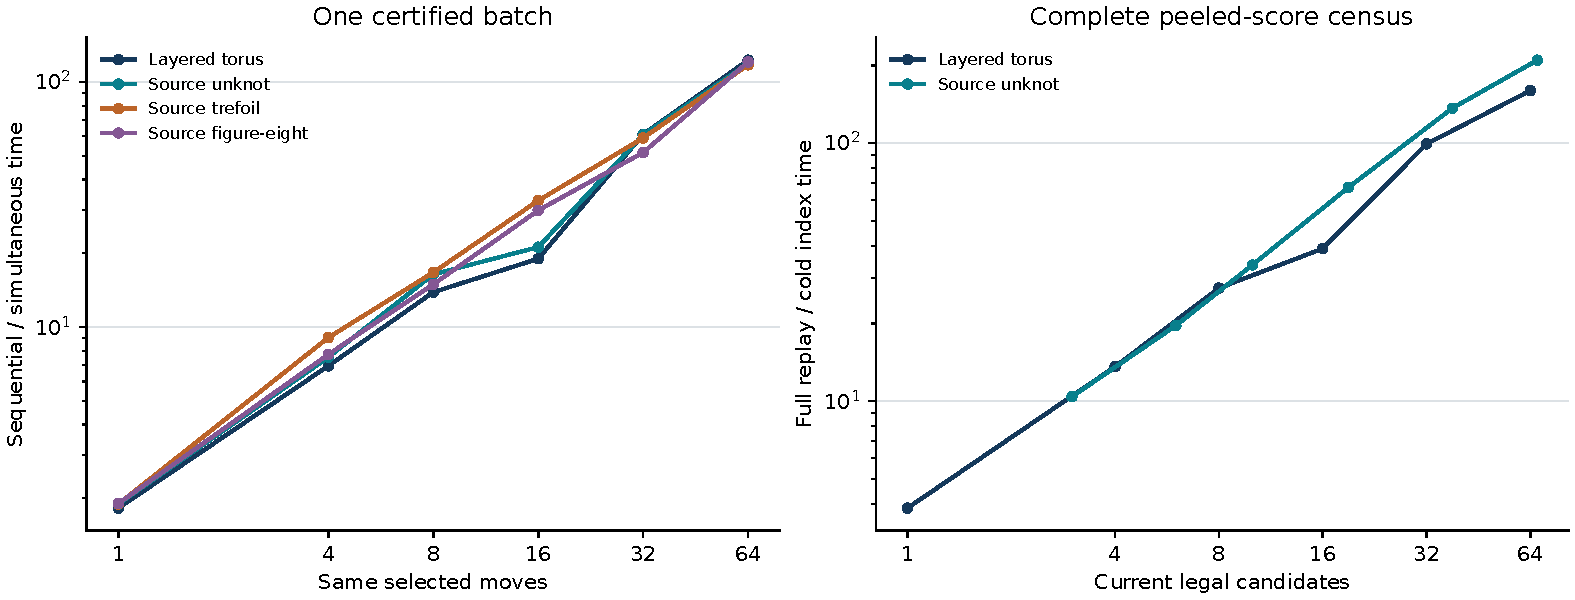
\includegraphics[width=\textwidth]{figures/geometric_performance.pdf}
\caption{Observed subroutine ratios, with three alternating paired rounds
per point. Left: simultaneous checked producer versus the existing literal
sequential composition on the same selected sites. Right: a freshly built
minima index and complete candidate census versus full individual geometric
replay of every candidate. Lines connect measured points; they are not
fitted asymptotic bounds.}
\label{fig:performance}
\end{figure}

\subsection{A cold index plus the entire peeled-score census}

This comparison starts the dynamic state from scratch on every timed run.
It includes the index construction and complete current candidate census.
The reference independently prepares the same input, performs every
candidate with the individual geometric producer and transport consumer,
and recomputes all vertex-link minima. The entire ordered list of site,
peeled Euler gain, and peeled piece saving agrees exactly. It is not a
comparison against a previously optimised static thirteen-prefix
implementation; the incoming report supplied a theorem for that pass,
not such an implementation.

\begin{table}[htbp]
\centering\small
\begin{tabular}{lrrrrrr}
\toprule
Family & Inserted sites & $t$ & Census $M$ & Full replay (s)& Cold index (s)& Ratio\\
\midrule
Layered &1&3&1&0.00135&0.00035&3.85\\
Layered &4&12&4&0.01738&0.00128&13.59\\
Layered &8&24&8&0.06480&0.00236&27.42\\
Layered &16&48&16&0.30292&0.00777&39.00\\
Layered &32&96&32&1.14917&0.01157&99.30\\
Layered &64&192&64&4.74531&0.02968&159.86\\
\midrule
Unknot &1&21&3&0.02030&0.00195&10.40\\
Unknot &4&24&6&0.04827&0.00246&19.62\\
Unknot &8&28&10&0.09583&0.00284&33.69\\
Unknot &16&76&19&0.50188&0.00745&67.37\\
Unknot &32&132&38&1.71692&0.01258&136.53\\
Unknot &64&204&67&5.09894&0.02432&209.69\\
\bottomrule
\end{tabular}
\caption{Complete peeled candidate scoring, including a fresh index on
the faster arm. The census can include legal sites beyond the inserted ones.}
\label{tab:peeling}
\end{table}

The tree-maintenance theorem concerns repeated local edits. These timings
test a more conservative cold-start query; they do not isolate an amortised
update speedup. A separate fresh-geometry audit checks 23 committed batches
and 45 moves across four families, including stable-vertex/fresh-root
bijections, link types, every triangle record, all thirteen-key prefixes,
and exact collective score agreement. All checks pass.

\subsection{The active-support lift reduces calls but loses elapsed time}

The active audit contains 20 partial-mask cases across seven genuine finite
triangulations. Seventeen have positive objective and compare complete
support discovery by efficient unary probes with the homogeneous lifted
query. The unary method skips coordinates whose activity is already
witnessed by an earlier LP point. This is therefore a meaningful small-LP
baseline, not an artificially padded fixed number of queries.

\begin{table}[htbp]
\centering\small
\begin{tabular}{lrrrrrr}
\toprule
Family & Masks & Unary calls & Lift calls & Unary (s) & Lift (s) & Lift/unary\\
\midrule
Fibonacci, $t=1$ &2&6&2&0.00177&0.01644&9.30\\
Fibonacci, $t=2$ &3&16&3&0.02559&0.21252&8.30\\
Fibonacci, $t=3$ &3&24&3&0.17221&1.22396&7.11\\
Fibonacci, $t=4$ &3&27&3&0.42699&4.12959&9.67\\
Branching torus, $t=5$ &3&31&3&0.68977&16.10012&23.34\\
Boundary attachment, $t=3$ &3&26&3&0.10197&1.14782&11.26\\
Finite trefoil, $t=5$ &3&3&0&0.22226&---&---\\
\bottomrule
\end{tabular}
\caption{Time sums across the specified masks. The last row terminates
after negative ordinary prechecks, so it does not run the lifted query.}
\label{tab:active-timing}
\end{table}

Across the 17 positive paired cases, the unary method uses 130 LP calls,
1,418 pivots, and 1.418307 seconds; the lift uses 17 calls, 1,449 pivots,
and 22.830456 seconds. The aggregate slowdown is 16.10-fold. The median
individual slowdown is 8.84-fold, the range is 5.89--38.48-fold, and the
lift wins no timing comparison. Similar pivot counts do not imply similar
work because the lifted tableau is much larger. These data support the
certificate interface but oppose enabling this dense implementation as a
general speed optimisation.

A separate exploratory direct lift of the unrestricted five-tetrahedron
trefoil root took 78.577357 seconds and 2,664 pivots to return nonpositive.
It is a single exploratory observation, not a repeated paired measurement.
The retained default audit uses a 25-second allowance per request and has
no cap outcomes. The ordinary precheck prevents this unnecessary lifted
query on the negative control.

\subsection{Complete search controls and independent replay}

\begin{table}[htbp]
\centering\small
\begin{tabular}{llrrrrr}
\toprule
Source & Precheck & Time (s) & Nodes & Branches & LP calls & Lifts\\
\midrule
Fibonacci 1 &yes&0.00105&3&0&3&0\\
Fibonacci 1 &no &0.04512&5&2&5&5\\
Fibonacci 2 &yes&0.17846&5&2&7&2\\
Fibonacci 2 &no &0.48030&6&3&6&6\\
Fibonacci 3 &yes&1.22946&6&3&9&3\\
Fibonacci 3 &no &3.29603&7&4&7&7\\
Finite trefoil &yes&2.45246&20&0&20&0\\
\bottomrule
\end{tabular}
\caption{Seven full anchored searches. The Fibonacci controls return
positive Euler; the finite trefoil proves no positive-Euler vector across
its 20 anchors. Every result has an independently replayed certificate.}
\label{tab:active-search}
\end{table}

The replay script checks 37 support certificates and all seven complete
normal-search certificates without importing an LP solver. Positive
meridian controls are additionally checked through the maintained
compressing-disc endpoint. The experimental active search does not include
the earlier mandatory-type propagation, so its branching on Fibonacci
inputs is not a measurement of the maintained recognizer's policy.
When no active query ran, an empty observed-rank statistic is not a proof
that the root rank is zero.

The final maintained-plus-overlay test run reports \fulltestcount{} tests
passing. It includes \focusedtestcount{} focused tests for the new
interfaces. Tests cover all 24 orders of four disjoint sites, all six
orders of three sites on each of three source exteriors, shared boundary
facets, true overlapping-star rejection, malformed/corrupted proofs,
producer-disabled consumer replay, exact large integer scales, callback
cancellation, and input immutability. Randomised algebraic audits compare
600 bounded matching instances with exhaustive search, including 300
small-cover cases with the general backend disabled. Three initial full-run
errors were missing historical fixture files; two byte-verified pinned
fixtures were restored, the affected tests passed, and the complete suite
was rerun. The retained logs distinguish that setup failure from the final
verified result.

